\section{Presentation and reverse proxy}\label{sec:reverse-proxy}
The second core submodule created for the purpose of collecting the data from the users is the frontend application exposed to the internet.
This can be split further into two different functional modules~--- client and server-side.

\subsection{Client side module}\label{subsec:client-side-module}
The client-side module is an end-user presentation layer that is built with the HTML5 and CSS3~--- technologies that are the core and standard for modern web applications nowadays.
HTML is a widely used markup language used to create hypertext documents and CSS is used as a style-sheet for modifying the design of web documents.
The content of the website is a free, prebuilt template taken from the Colorlib\upperref{itm:colorlib} collection which web templates are licensed under the CC BY 3.0 License\upperref{itm:license}.
The mechanism that collects users' mouse actions is designed as a "plugin" script, meaning that the template can be changed easily, so different styled environments that serve various purposes can be used to collect the data.

To use the system and participate in the research, an interested user is required to first accept the consents of usage of the website as well as accept the usage of the cookies and then registration is allowed and required, and afterward, the user is redirected to the login page.
To persists consistency of the registration and login, the custom static web pages were created to be easily transferable between the templates.
On each document, the FAQ panel with more information regarding the project is exposed as a drop-down list.
To authenticate, users are required to provide the credentials to log in to the system.
These credentials are then sent through https --- which means that they are secured and encrypted --- to the reverse proxy server which then performs some action to authenticate a user, sets the cookie with granted \gls{jwt} token and redirects the user to the homepage.
More on the user authentication and the token obtaining sequence is described in
The whole sequence is described and shown in subsection~\ref{subsec:server-side-module}).

After a successful login, the token allows for site usage and ensures the identity of the user.
From now on, the actions performed by the user are recorded into the batches and sent to the \gls{api} every two seconds.
The event listeners are awaiting four different action types: mouse move, mouse-down, mouse-up, mouse wheel action.
Collected actions are packed into \gls{json} object and sent to the server side \gls{api} (described in~\ref{subsec:server-side-module}) --- the fields included are shown in the Listing~\ref{listing:mouse-events-json-schema}.

\begin{listing}[H]
    \inputminted[
    linenos,
    autogobble,
    xleftmargin=0.7cm,
    xrightmargin=0.7cm,
%    frame=single,
    framesep=2mm,
    labelposition=bottomline,
    baselinestretch=1.2,
    fontsize=\footnotesize
    ]{json}{resources/mouse-event-json-schema.json}
    \caption{JSON schema for mouse event batches}
    \label{listing:mouse-events-json-schema}
\end{listing}

\subsection{Server side module}\label{subsec:server-side-module}
The server side module is build with Node.js\upperref{itm:node} runtime with the Express\upperref{itm:express} framework on the top of it.
Node.js is an asynchronous JavaScript runtime, which is widely used to build high-end, scalable commercial applications.
Express is light-weight and simple to use, yet powerful web framework for Node.js, which allows for a fast and convenient HTTP server set-up server for serving the static web documents over the internet.
This module is serving the purpose of reverse proxy between clients and the backend \gls{api}.

The main responsibilities of the reverse proxy are signing up the user, token granting, validation and caching, serving static web documents storing and passing the data to for persistence.
When a new user tries to sign-up, secured with \gls{tls} (Transport Layer Security) credentials from the sign-up form are sent to one of the proxy endpoints, where they are then passed to the backend \gls{api}.
Because the backend is not exposed anywhere over the public network, there is no need to secure the credentials with \gls{tls}.\\
The user is granted \gls{jwt} Access and Refresh tokens after logging in using the login form.
The user credentials are secured with \gls{tls} and received by proxy \gls{api}, whereas the proxy server is additionally appending the Client id and Client secret for OAuth2 server to the request "Authorization" header, as the proxy server authenticates to OAuth2 server with HTTP Basic authentication scheme.

Credentials of the user that wishes to log in are included in the body of the request.
When the user is properly authenticated, the OAuth2 server responds with a valid \gls{jwt} token which is then set as a cookie with HttpOnly, Secure, and SameSite strict options.
When the token is successfully granted, it is also saved to the Redis, which is a simple to use key-value NoSQL database suitable for caching.
The retrieval of such a token is very fast, so this is serving the purpose of the caching system, which results in a great efficiency improvement and lower response time of the server.
For each interaction and request for resources, the user has to hold a valid \gls{jwt} Token.
First, the token is searched in the cache database.
If it does not figure there, the proxy server is attempting to check the token with the backend OAuth2 server.
If the server responds with Bad Request status or the access token is not set on the user request, the refresh token is being used for access token renewal.
The complete sequence visualization can be seen in \mbox{Fig.~\ref{fig:jwt-sequence}}.
The proxy server is storing the user mouse data received from the client side and periodically passes it to the backend \gls{api} for persistence.




% Propably should be included elsewhere, maybe appendix?
\begin{figure}[!hbt]
    
    \centering
    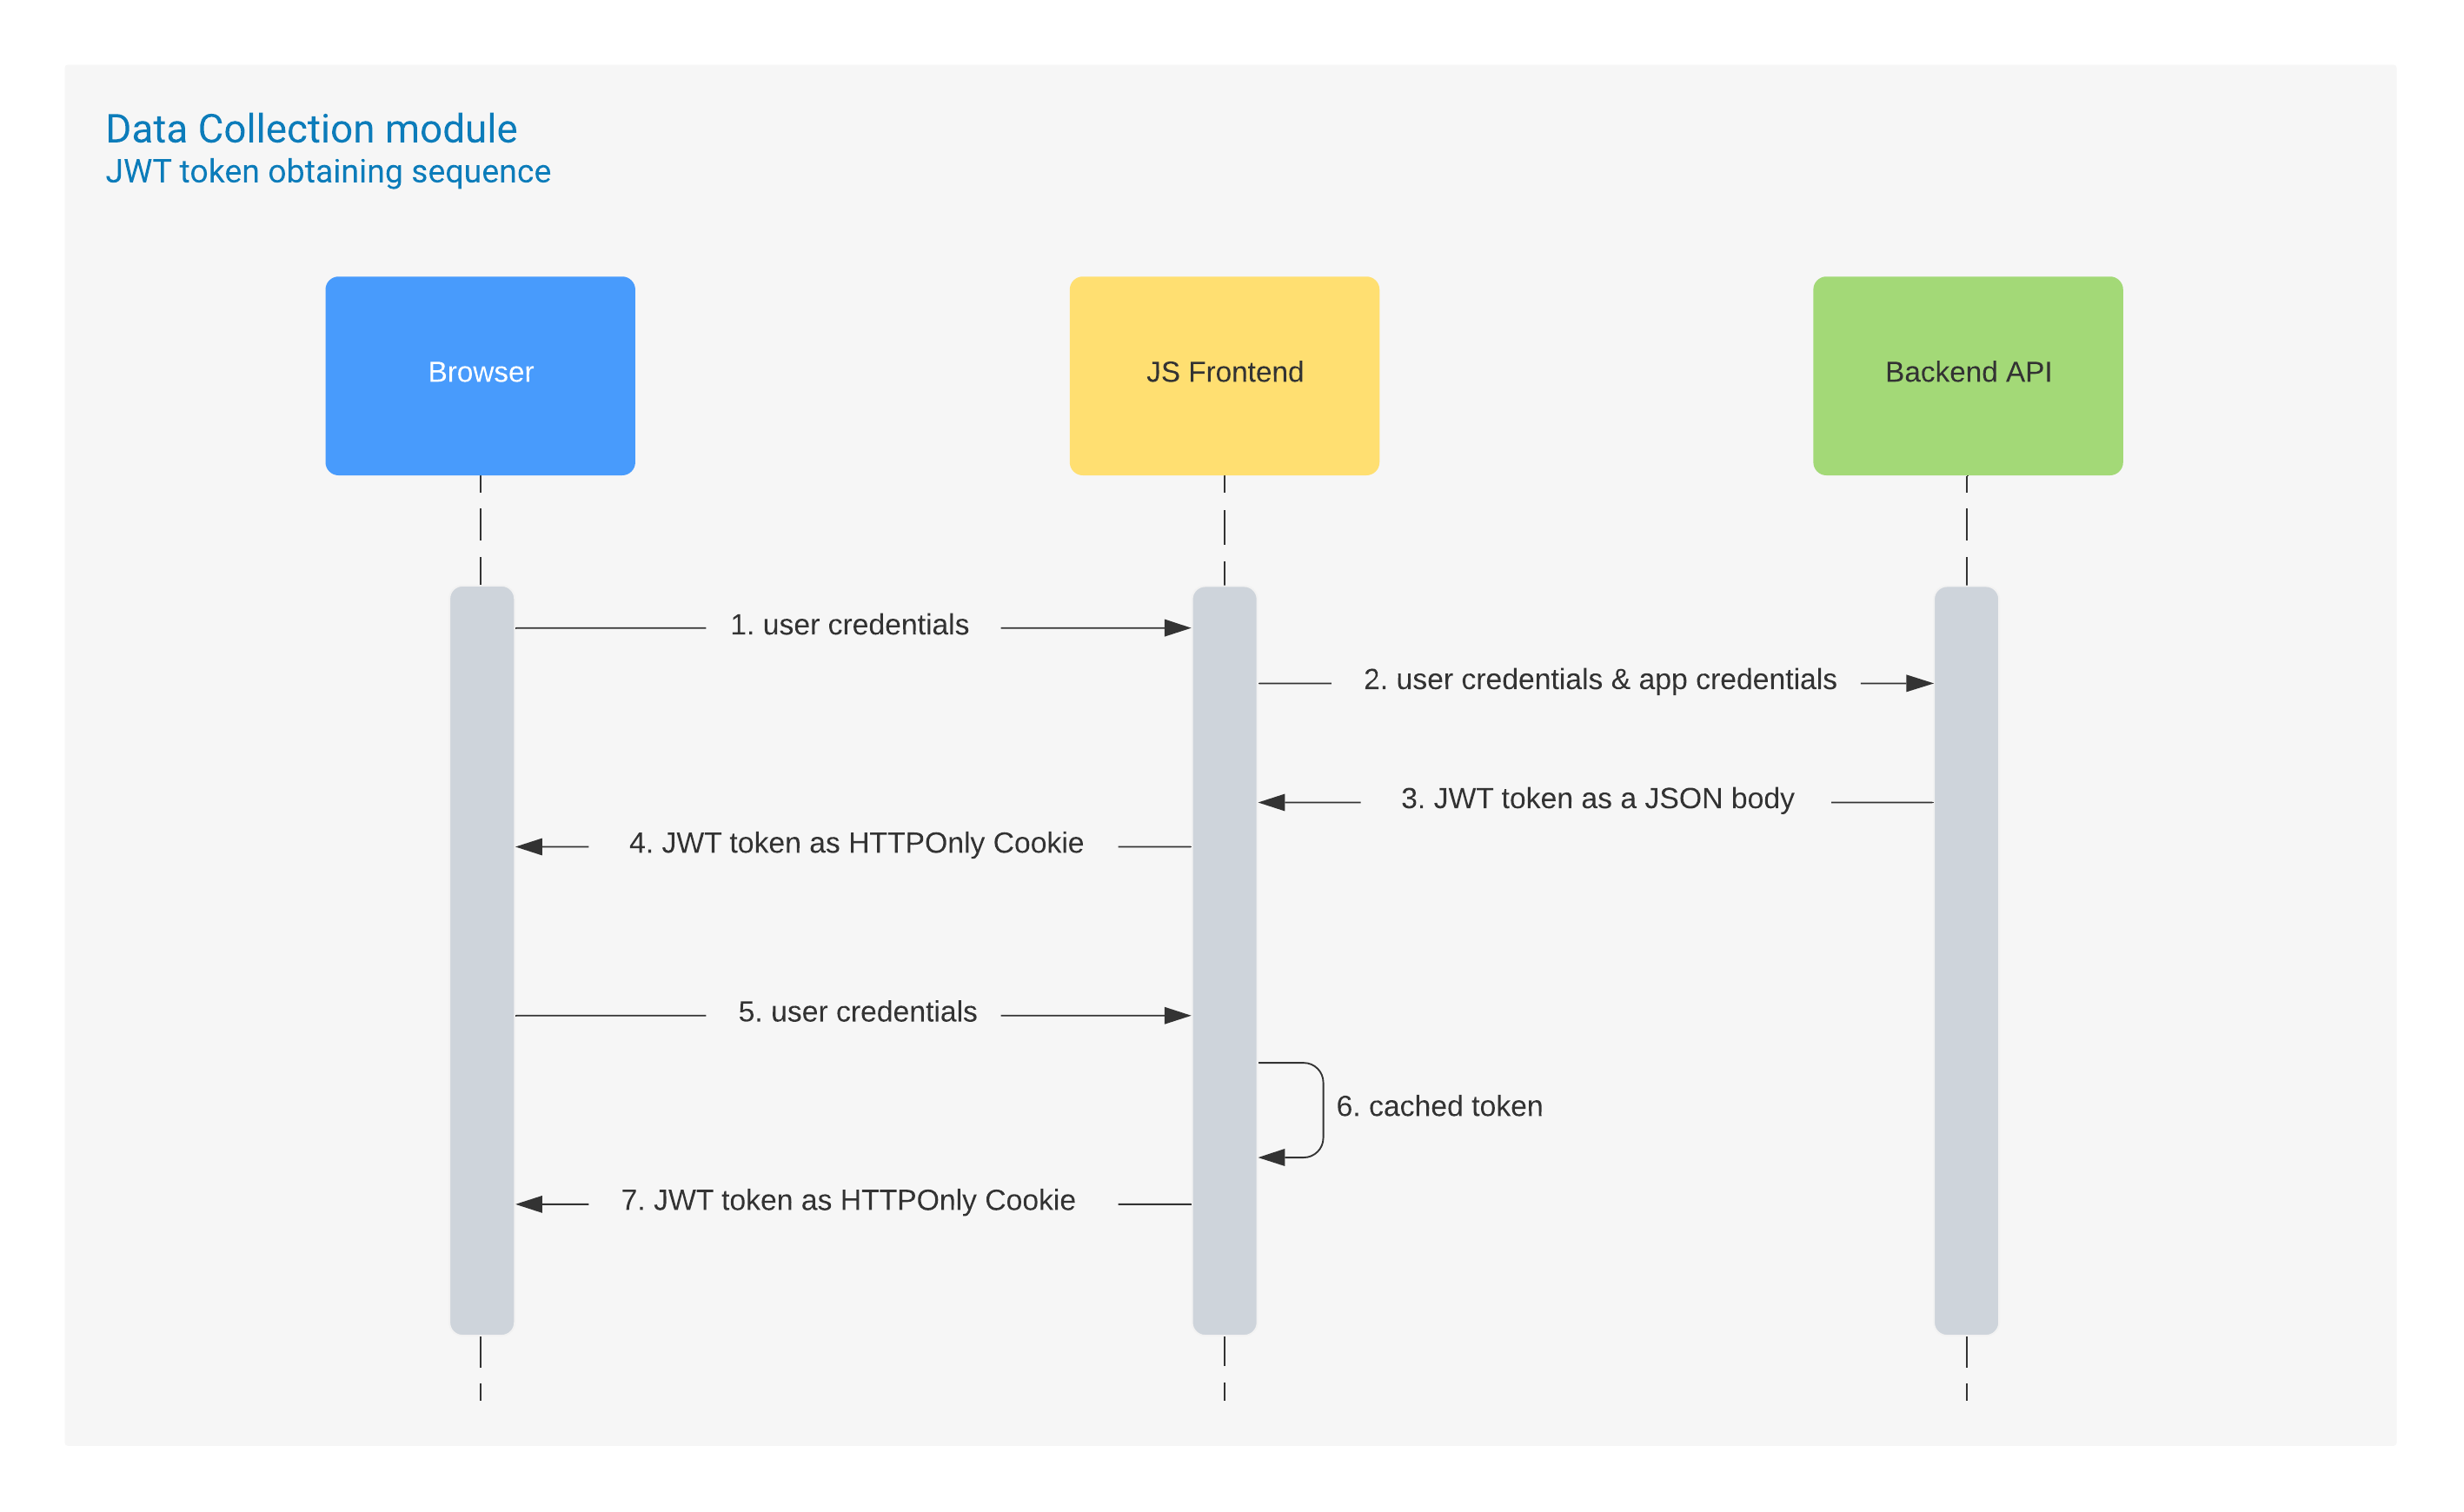
\includegraphics[width=\linewidth]{resources/jwt_sequence_diagram.png}
    \captionsetup{width=\linewidth}
    \captionof{figure}{JWT token obtaining sequence}
    \label{fig:jwt-sequence}
\end{figure}